\documentclass[8pt]{beamer}
%\usepackage{comment}
\usepackage{style}
\title[ Proyecto Junior PIJ-15-19]{  Estudio de la distribución de hidrógeno fotoionizado en el Centro Galáctico }
\author[Dr. Ericson López, Jr. Jairo Armijos, et. al.]{\large	 Dr. Ericson López, Jr. Jairo Armijos, et. al. \\ \vspace{0.2cm}
GRUPO DE RADIOASTRONOMÍA \\ \vspace{0.2cm} OBSERVATORIO ASTRON\'OMICO DE QUITO}
\date{Quito, noviembre 2019.}
\begin{document}
\begin{frame}
\rule[0.05mm]{162mm}{0.05mm}
\begin{minipage}[d]{30mm}
\begin{center}

\includegraphics[scale=.20]{logo_epn.eps}
\end{center}
\end{minipage}
\begin{minipage}[d]{60mm}
\begin{center}
\vspace{0.2cm}
\textsf{\textbf{ ESCUELA POLIT\'ECNICA NACIONAL }}\\
\textsf{\textbf{ \small OBSERVATORIO ASTRON\'OMICO DE QUITO }}
%\textsf{\textbf{\tiny  Grupo de Cosmolog\'ia y Relatividad General}}\\
\end{center}
\end{minipage}
\begin{minipage}[d]{30mm}
\begin{center}

\includegraphics[scale=.55]{oaq.png}
\end{center}
\end{minipage}\\
\rule[1mm]{162mm}{0.20mm}
\maketitle
\end{frame}
\begin{frame}
\frametitle{Contenido:}
\tableofcontents
\end{frame}
\begin{frame}
\frametitle{Campos magnéticos en las afueras de  galaxias}
\section{Campos magnéticos en las afueras de  galaxias}
\textbf{Resumen:}\\
Utilizando datos públicos de monóxido de carbono(CO), se estudiaron las condiciones de excitación del CO y la intensidad de campo magnético de  cuatro galaxias espirales. 
Para las afueras de las galaxias se encontraron:
\begin{itemize}
\item Temperaturas cinéticas $\lesssim 35-38K$ 
\item Densidades de columna de CO $\lesssim 10^{15}-10^{16}cm^{-2}$
\item Masas de hidrógeno molecular $H_2$ $\lesssim 4\times 10^{6}-6\times 10^{8}M_{\odot} $ \item La intensidad de campo magnético  $\lesssim 6-31 \mu G$ 
\end{itemize}
\begin{center}
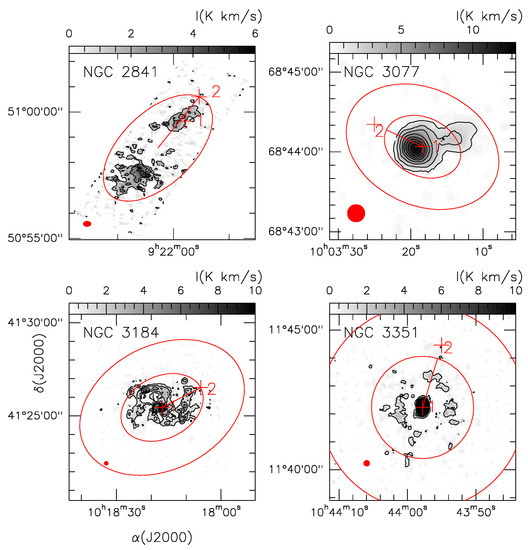
\includegraphics[width=0.3\linewidth]{figures/galaxies.jpg}
\captionof{figure}{Mapa de intensidad integrada de CO(2-1) de las cuatro galaxias estudiadas }
\end{center}
\end{frame}
\begin{frame}
\frametitle{Metodología}
Para el estudio del campo magnético se utiliza el método de Dotson que permite obtener una ecuación magnetohidrodinámica simplificada. Esta ecuación permite hallar una cota de intensidad de campo magnético $B$:
\begin{equation*}
    B<3.23\times 10^{-8}\left(\frac{R}{pc}\right)^{0.5}\left(\frac{n}{cm^{-3}}\right)^{0.5}\left(\frac{M}{M_{\odot }}\right)^{0.5}\left(\frac{r}{pc}\right)^{-1}
\end{equation*}
donde $R$ es el radio de las líneas de campo magnético, $n$ la densidad del hidrógeno molecular, $M$ y $r$ la masa total y el radio de la galaxia. En el estudio se usaron mediciones de CO(2-1) obtenidas con el telescopio IRAM 30m a $230GHz$ y una resolución espacial de 13 segundos de arco.
\begin{center}
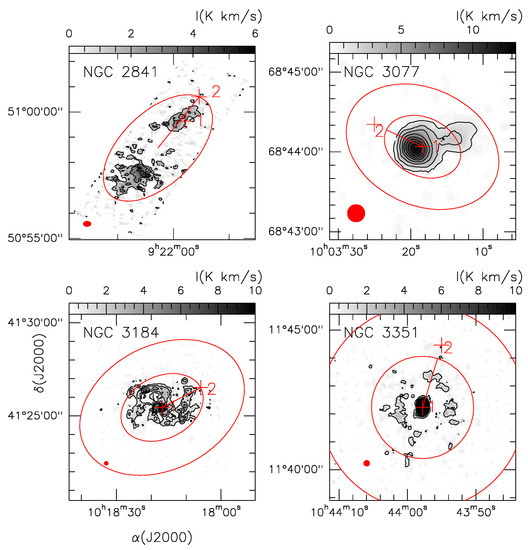
\includegraphics[width=0.3\linewidth]{figures/galaxies.jpg}
\captionof{figure}{Mapa de intensidad integrada de CO(2-1) de las cuatro galaxias estudiadas }
\end{center}
\end{frame}
\begin{frame}
\frametitle{Resultados }
La masa de hidrógeno $M_{H_2}$ para la galaxia y sus afueras se derivó usando la expresión
\begin{equation*}
    \dfrac{M_{H_2}}{M_{\odot}}=5.5\dfrac{R_{21}}{0.8}\left(\dfrac{L_{CO}}{Kkms^{-1}pc^2}\right)
\end{equation*}
donde $R_{21}$ es un cociente de intensidad de línea $CO(2-1)/CO(1-0)$ y $L_{CO}$ es la luminosidad de CO..La masa en las afueras de las galaxias es $\lesssim 4\times10^{6}-1\times10^{9}$ masas solares.\\

\textbf{Campo magnético en las galaxias y sus afueras}


\begin{center}
\begin{tabular}{ c c c } 
\hline
Galaxia& Región & B$(\mu G)$\\
 \hline
 NGC2841 & Disco & $\lesssim31$ \\
  & Afueras & ... \\
\hline
 NGC3077 & Disco & $\lesssim 6$ \\ 
   & Afueras & $\lesssim 7$ \\
 \hline
 NGC3184 & Disco & $\lesssim 14$ \\
   & Afueras & $\lesssim 19$ \\
\hline
 NGC3351 & Disco & $\lesssim 11$ \\
   & Afueras & $\lesssim 15$ \\

 \hline
\end{tabular}
\end{center}
\end{frame}
\begin{frame}
\frametitle{Conclusiones}
\begin{itemize}
    \item La intensidad de campo magnético estimada es $\lesssim 6-31\mu G$ que son consistentes con aquellas de  $\sim 20-60\mu G$ observadas en galaxias espirales.
    %Este resultado sugiere que el polvo es la principal componente que influencia el campo magnético en comparación con el gas molecular.
    \item En las afueras de las galaxias, la temperatura cinética es $\lesssim 35-38K$, la densidad de columna  de CO$\lesssim 10^{15}-10^{16}cm^{-2}$, la masa $M_{H_2}$ $\lesssim4\times10^6-6\times 10^{8}$ masas solares y la densidad de hidrógeno $\lesssim10^3cm^{-3}$.  
\end{itemize}
\end{frame}
\begin{frame}
\frametitle{Cinemática y masa de la Galaxia NGC7331}
\section{Cinemática y Masa de la Galaxia NGC7331}
\textbf{Resumen:}\\
Se estudió la curva de rotación de la galaxia NGC 7331, usando observaciones del monóxido de carbono (CO). La forma de la curva de rotación y las velocidades son similares a las derivadas previamente, empleando datos de hidrógeno atómico, esto sugiere la coexistencia de ambos elementos en las regiones estudiadas en NGC 7331. \\
Asimismo, se estudió el campo de velocidades del gas, lo que puso en evidencia la rotación de la galaxia en sentido horario. Finalmente, se estimó una masa dinámica de 1,4E+10 masas solares para NGC 7331. 
\begin{center}
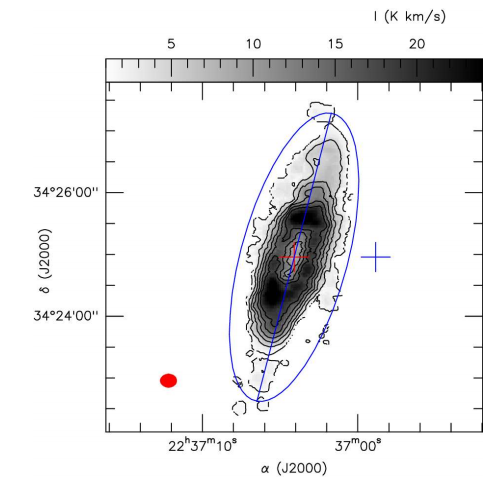
\includegraphics[width=0.4\linewidth]{figures/ngc7331_1.png}
\captionof{figure}{\footnotesize{Mapa de intensidad integrada de CO (2-1) de NGC 7331.}   }
\end{center}
\end{frame}
\begin{frame}
\frametitle{Análisis de datos}
NGC 7331 es una galaxia espiral cercana, situada a 14.7 Mpc de la Tierra. En el estudio se usaron datos de CO (2-1) observados a  230.5GHz y una resolución espacial de 13 segundos de arco. \\
\textbf{ MAPA Y ESPECTROS DE LA GALAXIA NGC 7331 }\\
\begin{minipage}[t]{0.32\linewidth}
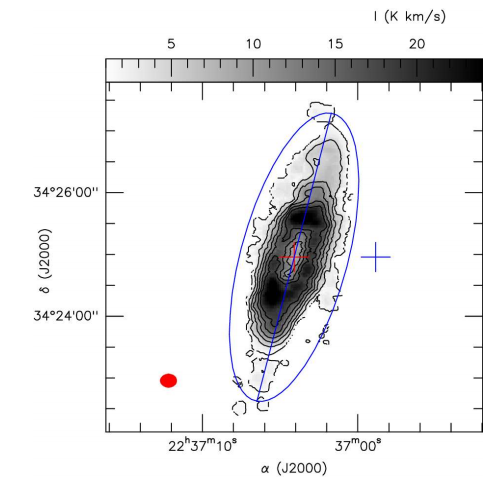
\includegraphics[width=0.9\linewidth]{figures/ngc7331_1.png}
\captionof{figure}{\footnotesize{Mapa de intensidad integrada de CO (2-1) de NGC 7331.}   }
\end{minipage}
\begin{minipage}[t]{0.32\linewidth}
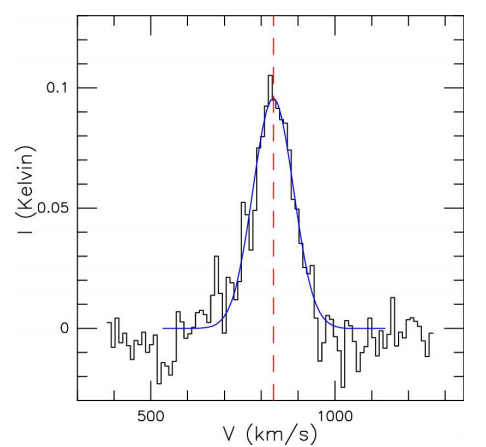
\includegraphics[width=0.8\linewidth]{figures/ngc2.png}
\captionof{figure}{ \footnotesize{Espectro de emisión de CO (2-1) del centro de NGC 7331.} }
\end{minipage}
\begin{minipage}[t]{0.32\linewidth}
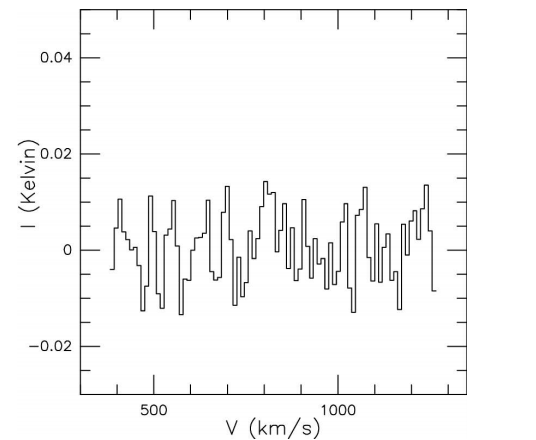
\includegraphics[width=0.9\linewidth]{figures/ngc3.png}
\captionof{figure}{\footnotesize{Espectro observado en una posición alejada  del centro de NGC 7331. Indicada con una cruz azul en el mapa.}}
\end{minipage}	
\end{frame}
\begin{frame}
\frametitle{Resultados y Conclusiones}
\textbf{CURVA DE ROTACIÓN}\\
Una curva de rotación muestra la velocidad del gas en función de una posición. La curva de rotación de NGC7331 se muestra abajo.
\begin{center}
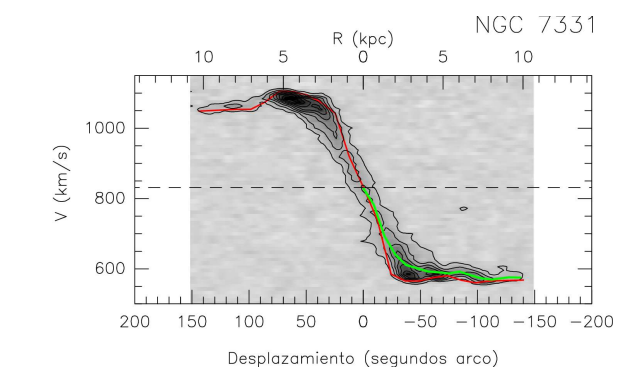
\includegraphics[width=0.450\linewidth]{figures/rotacion.png}
\captionof{figure}{ Las líneas rojas y verdes representan velocidades de rotación de NGC7331.}
\end{center}
\textbf{CONCLUSIONES}\\
\begin{itemize}
\item La forma de la curva de rotación y las velocidades de NGC 7331 derivadas a partir de observaciones de CO (2-1) son muy similares a aquellas derivadas usando el hidrógeno atómico. Este resultado sugiere la coexistencia del gas de monóxido de carbono e hidrógeno atómico en las regiones estudiadas.
\item La galaxia NGC 7331  rota en sentido horario. 
\item La masa dinámica derivada para la galaxia NGC7331 es de 1,4E+10 masas solares. 
\end{itemize}
\end{frame}
\begin{frame}
\frametitle{Gas ionizado difuso en corrientes de gas cerca de Sgr $A^*$}
\section{Gas ionizado difuso en corrientes de gas cerca de Sgr $A^*$}
\textbf{Resumen:}\\
Se llevó a cabo un estudio del gas ionizado difuso hacia tres posiciones de nubes ubicadas en el Centro Galáctico: $20kms^{-1}(LOS-0.11)$, $50kms^{-1}(LOS-0.02)$ y $LOS+0.693$. La emisión del gas ionizado se detectó mediante las líneas de recombinación $Hn\alpha$ y $Hn\beta$. Se derivan propiedades físicas y cinemáticas de las fuentes. Se halló la fracción de masa de He a H  de $0.29\pm 0.01$ que sustenta  la idea que las estrellas masivas en el Centro Galáctico han aumentado la abundancia de helio en comparación con su valor primordial.
\begin{center}
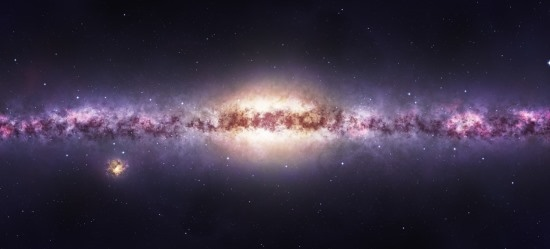
\includegraphics[width=0.6\linewidth]{figures/galactic_centre.jpg}
\captionof{figure}{\footnotesize{Imagen del Centro de la Vía Láctea.}   }
\end{center}
\end{frame}
\begin{frame}
\frametitle{Observación y análisis de datos.}
La observación fue realizada con el telescopio Green Bank de 100m de NRAO  en el 2009, con una resolución espacial de 24.4KHz. También se utilizaron datos del archivo de NRAO del VLA a 24.5GHz. La siguiente gráfica muestra las posiciones observadas en las tres fuentes.
Las líneas de recombinación de hidrógeno (H) y Helio (He) fueron identificadas mediante el catálogo disponible en el software MADCUBA[1].
%que contiene las frecuencias estimadas de acuerdo a la teoría de Dirac.
Las fuentes  $LOS-0.11$, $LOS-0.02$ muestran dos componentes de velocidad mientras $LOS+0.693$ presenta una sola. Algunas líneas identificadas se muestran en la siguiente gráfica:\\
%\vspace{0.3em} % When there are two boxes, some whitespace may need to be added if the one on the right has more content
\begin{minipage}[t]{0.50\linewidth}
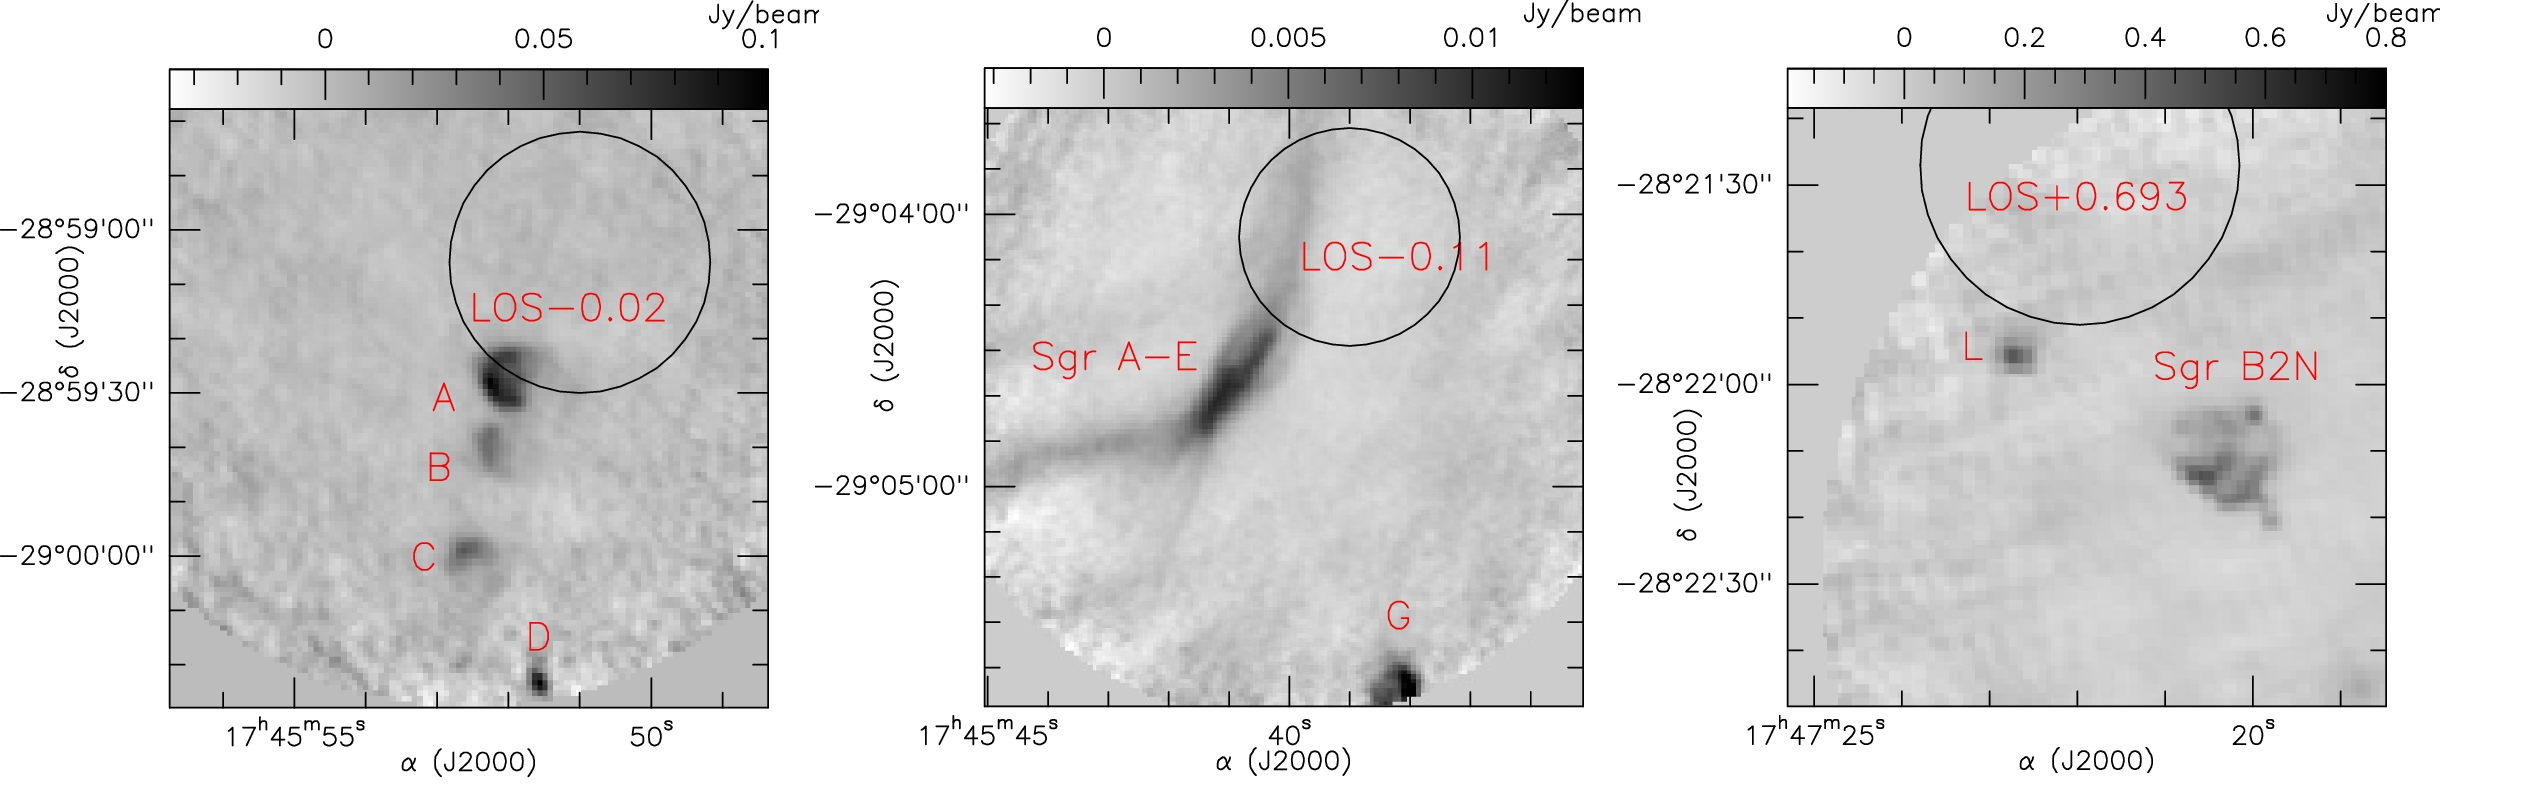
\includegraphics[width=\linewidth]{figures/los1.png}
\captionof{figure}{Mapa de radio continuo VLA a 24.5GHz de las tres posiciones observadas }
\end{minipage}
\begin{minipage}[t]{0.24\linewidth}
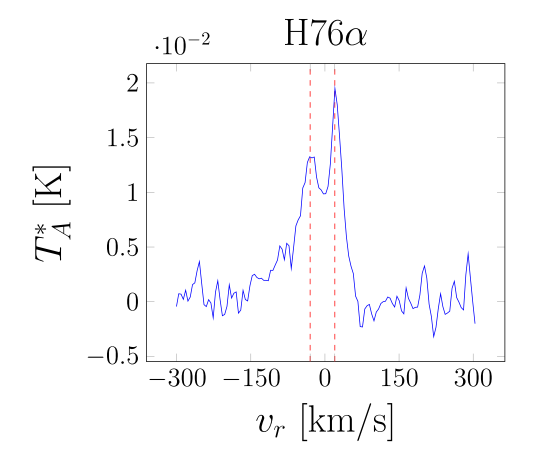
\includegraphics[width=0.95\linewidth]{figures/rrl1.png}
\captionof{figure}{ \footnotesize{Línea de hidrógeno en LOS-0.11} }
\end{minipage}
\begin{minipage}[t]{0.24\linewidth}
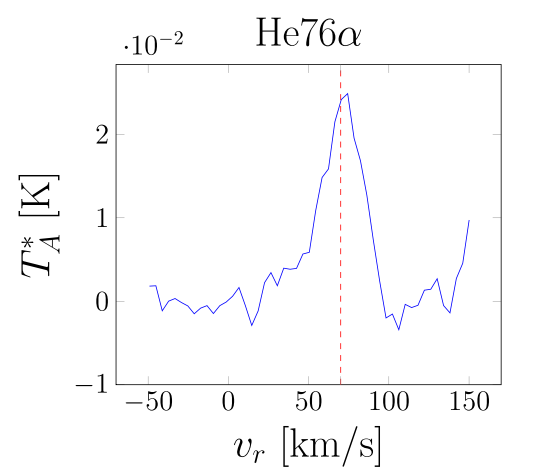
\includegraphics[width=0.95\linewidth]{figures/rrl2.png}
\captionof{figure}{\footnotesize{Línea de Helio en LOS+0.693}}
\end{minipage}
\end{frame}
\begin{frame}
\frametitle{Resultados.}
El gas ionizado difuso presenta velocidades positivas y negativas  en las fuentes LOS-0.11 y LOS-0.02. En la figura se muestran las velocidades de ambas fuentes en un diagrama posición-velocidad para la emisión CII, así como cuatro corrientes del gas del modelo de Kruijssen$[2]$. 
\begin{center}
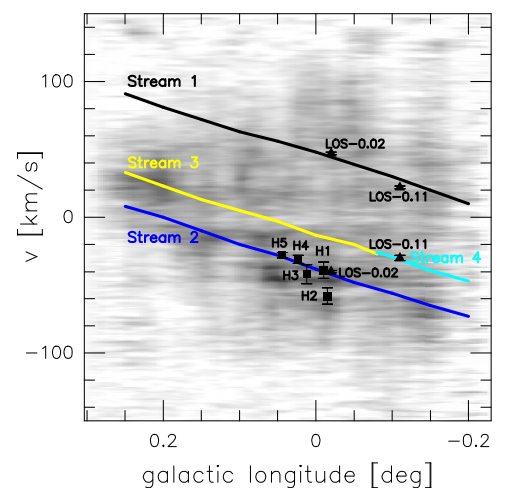
\includegraphics[width=0.55\linewidth]{figures/rrl4.png}
\captionof{figure}{Diagrama posición- velocidad para la emisión CII de las fuentes en escalas de grises. Las velocidades de las fuentes se muestran con estrellas y cuadrados. Las corrientes de gas se indican con líneas.}
\end{center}
\end{frame}
\begin{frame}
\frametitle{Conclusiones}
\begin{itemize}
    \item Se detectaron líneas de emisión $Hn\alpha$ con $n=79-75$, $Hn\beta$ con $m=99-96$,$94$ en dirección a $LOS-0.11$,$LOS-0.02$. Para $LOS+0.693$ también se detectó $H95\beta$. 
    \item El gas ionizado observado hacia las tres fuentes es emititido bajo condiciones de equilibrio termodinámico local. Ello gracias a la comparación de las observaciones con modelos.
    \item Para $LOS-0.11$, $LOS-0.02$ y $LOS+0.693$ se determinaron  las densidades electrónicas de $\sim 40-310cm^{-3}$
\end{itemize}
\end{frame}
\begin{frame}
\frametitle{La distribución de HI en el halo de la Vía Láctea.}
\section{La distribución de HI en el halo de la Vía Láctea.}
\textbf{Resumen:} 
Se  estudió de  la distribución espacial del gas HI en una región $80^{\circ}\times 90^{\circ}$ del halo de la Galaxia mediante observaciones de la línea de emisión de $21cm$ de hidrógeno(HI). Para la región estudiada se estimaron densidades de columna en el rango de $3-11\times 10^{20}cm^{-2}$.\\

Asimismo, en el mapa obtenido con una sensibilidad espectral de $\sim 2K$ , no se detectó ninguna línea de emisión de HI de $21cm$ por encima de dos veces el ruido en latidudes galácticas superiores a $\sim 46^{\circ}$
\end{frame}
\begin{frame}
\frametitle{Observación y análisis de datos}
El hidrógeno atómico neutro(HI) es el elemento más abundante del medio interestelar y su transición de 21cm permite trazar la estructura y la dinámica de la Vía Láctea.\\

Se mapeó una región entre las longitudes galácticas $87^\cir-180^\circ$ y latitudes galácticas $13^\circ-85^\circ$, en pasos de $5.5^\circ$. Las observaciones fueron realizadas el 2016, con dos radio telescopios del Observatorio Espacial Onsala y una resolución espacial de $6^{\circ}$ a 21cm.
\begin{center}
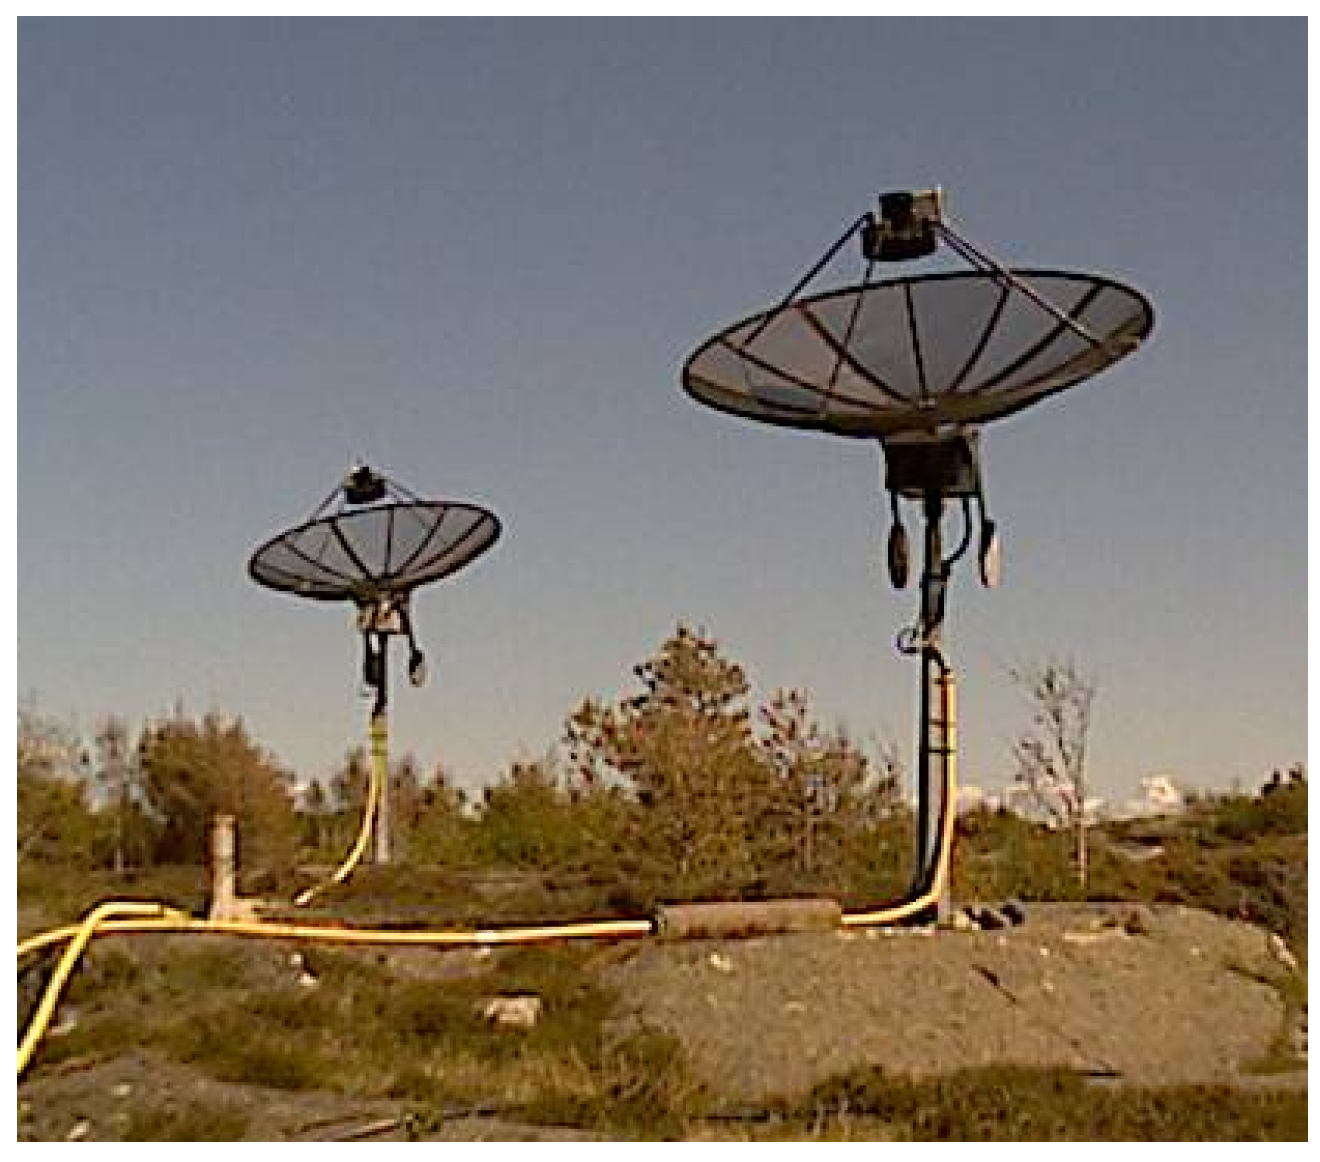
\includegraphics[width=0.3\linewidth]{figures/onsala.png}
\captionof{figure}{\footnotesize{Radio telescopios de $2.3m$ del Observatorio Espacial Onsala.}   }
\end{center}
El análisis y procesamiento de datos se realizó con el software SalsaSpectrum. El espectro de HI de 21cm obtenido fue comparado con espectros calibrados de las mismas posiciones galácticas que se observaron previamente por otros autores.

\end{frame}
\begin{frame}
\frametitle{Resultados}
Las líneas de emisión de HI 21cm más intensas fueron detectadas en latitudes galácticas más bajas$(\sim 8^\circ)$. En la gráfica se muestran los perfiles de emisión de HI 21cm observadas en tres diferentes posiciones de la Vía Láctea.
\begin{center}
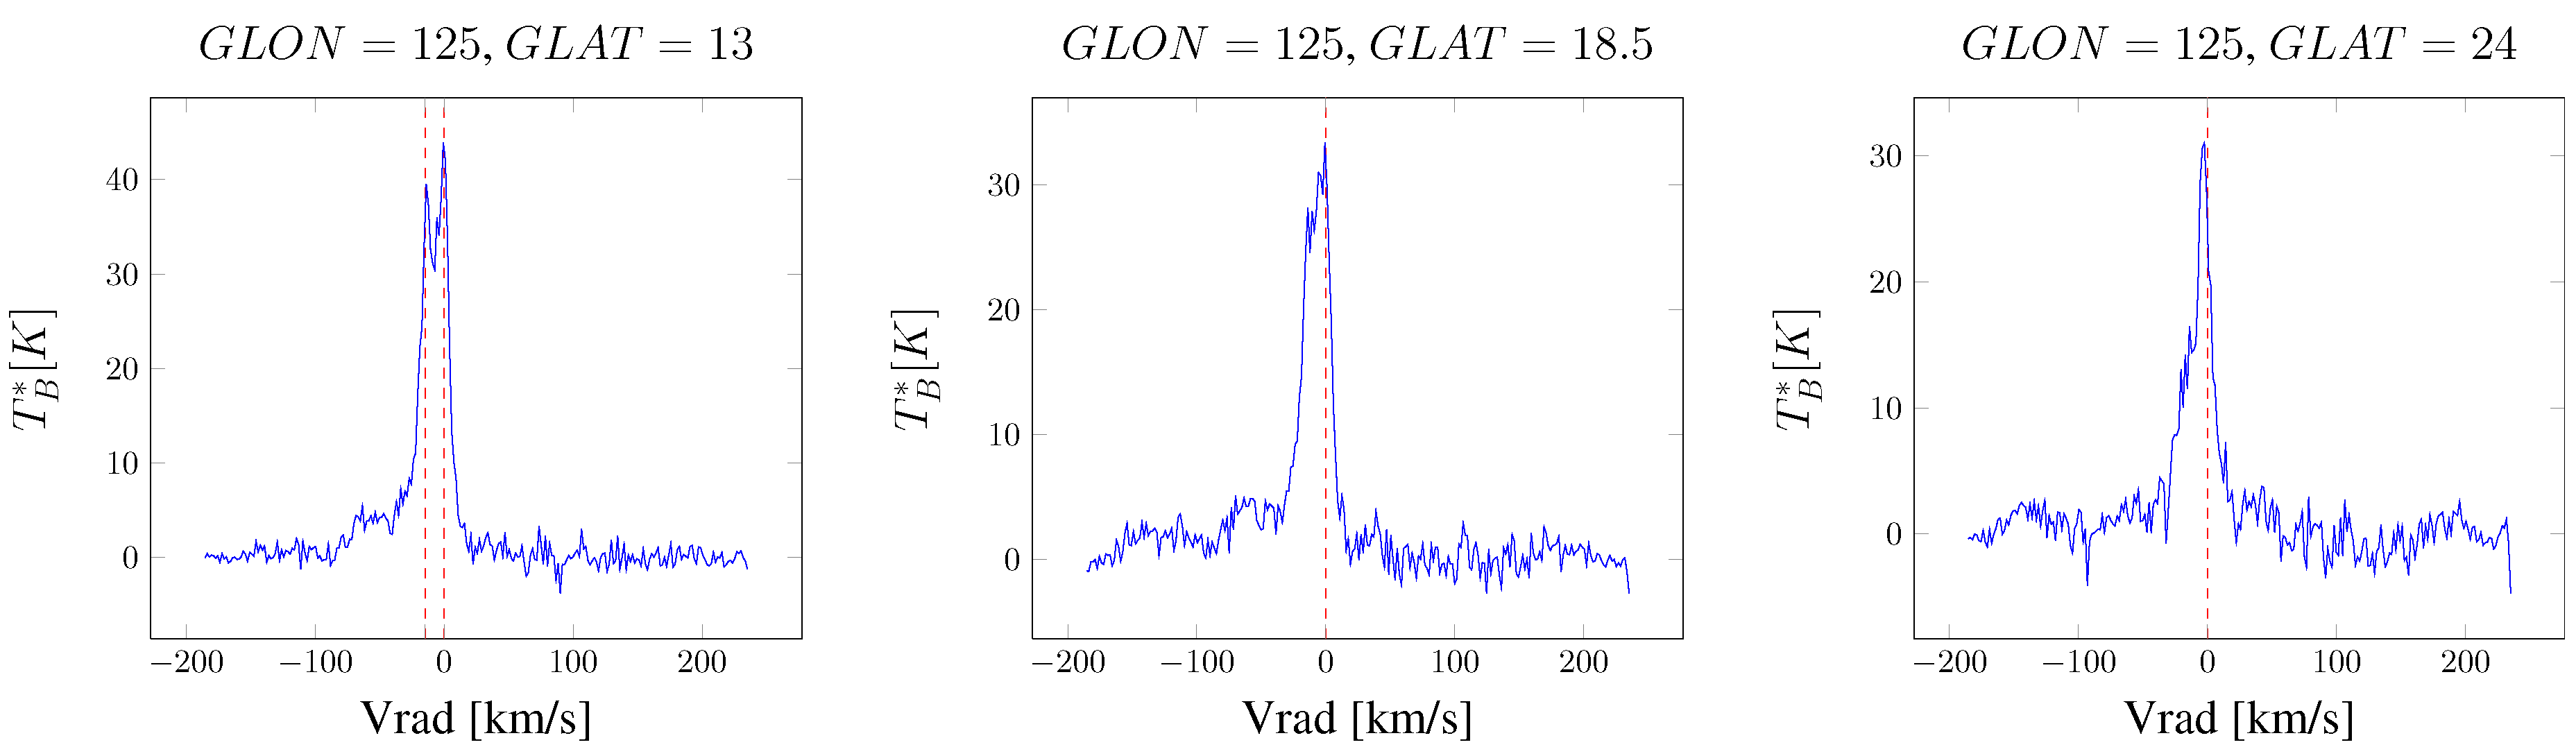
\includegraphics[width=0.7\linewidth]{figures/halo2.png}
\captionof{figure}{Líneas de emisión de HI 21cm observadas en tres posiciones diferentes en la Vía Láctea}
\end{center}
El mapa de intensidad máxima de la línea de HI 21cm muestra que esta no fue detectada por encima de $2\sigma$ $(\sigma=2K)$ para latitudes gálacticas superiores a $\sim 46\circ$.
\begin{center}
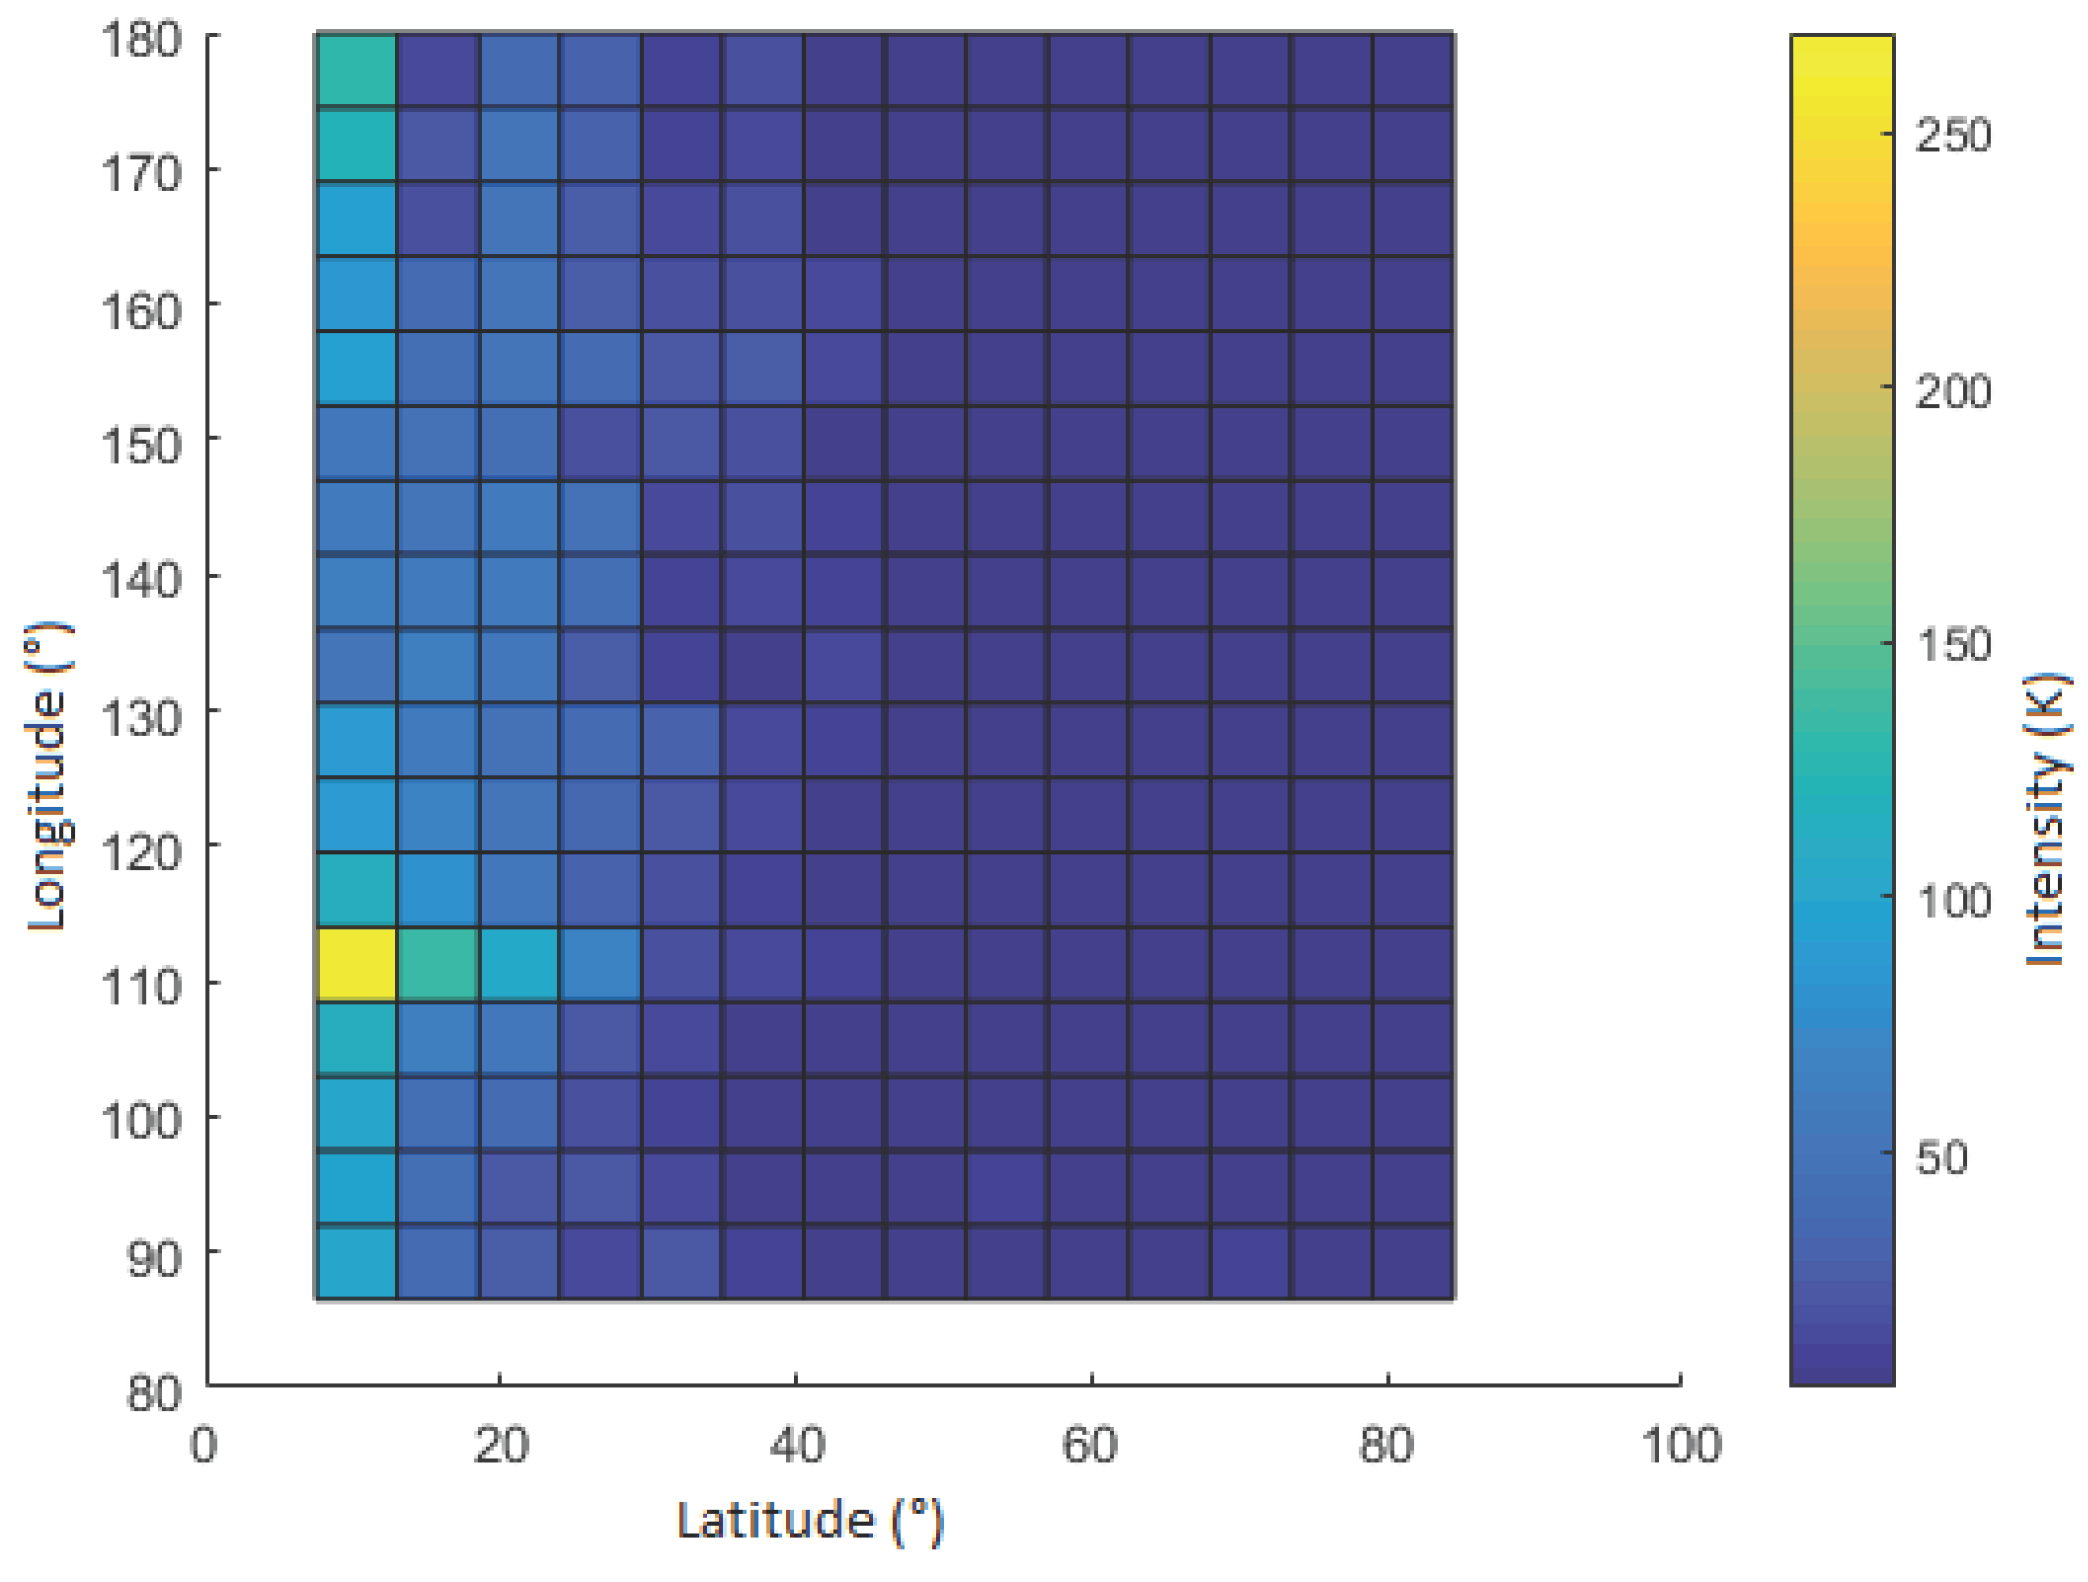
\includegraphics[width=0.4\linewidth]{figures/milky2.png}
\captionof{figure}{Mapa de intensidad de HI 21cm en la región $80^\circ-90^\circ$ de la Vía Láctea.}
\end{center}
\end{frame}
\begin{frame}
\frametitle{Conclusiones}
\begin{itemize}
  \item Obtuvimos un mapa de intensidad máxima de la línea de emisión HI de 21 cm para una región de $80^\circ \times 90^\circ$ de la Vía Láctea.
\item La densidad de columna de HI estimada $3-11\times10^{20}cm^{-2}$ es consistente con los valores previstos para las mismas regiones estudiadas con un instrumento de mayor resolución angular. 
\end{itemize}
\end{frame}
\end{document}